\chapter{Theoretical concepts}\label{cha:theory}

In \autoref{cha:theory} we will talk about theory. We start with lorem ipsum in \autoref{sec:this_a_sec}. Then continue with \molyd and \wolyd in \autoref{subsec:theorie_PL} and so on.
% Our text is \printinunitsof{in}\prntlen{\textwidth}\\ wide! % needs \usepackage{layouts}

\section{Referencing figures}\label{sec:this_a_sec}

In \autoref{fig:MoS2_schematic} one can see some nice pictures.


\unpacklipsum[2]\lipsumexp

\begin{figure}[t]
	\includegraphics[width=1\textwidth,keepaspectratio=true]{Images/MoS2_2.pdf}
	\caption[]{\textbf{(a)} Nice picture 1 \textbf{(b)}Nice picture 2}
	\label{fig:MoS2_schematic}
\end{figure}

\subsection{Stuff with \texorpdfstring{\moly}{MoS2} and \texorpdfstring{\woly}{WS2}}\label{subsec:theorie_PL} % \textorpfdstring needed to handle math symbols in section names and give ASCII alternative

\unpacklipsum[1-1]{}\lipsumexp

\subsection{Next section}\label{sec:next_sec}

One can also show figures where they where plaaced in the tex file or if not possible on top etc. by giving [!ht] as arguments.

\begin{figure}[!htb]
	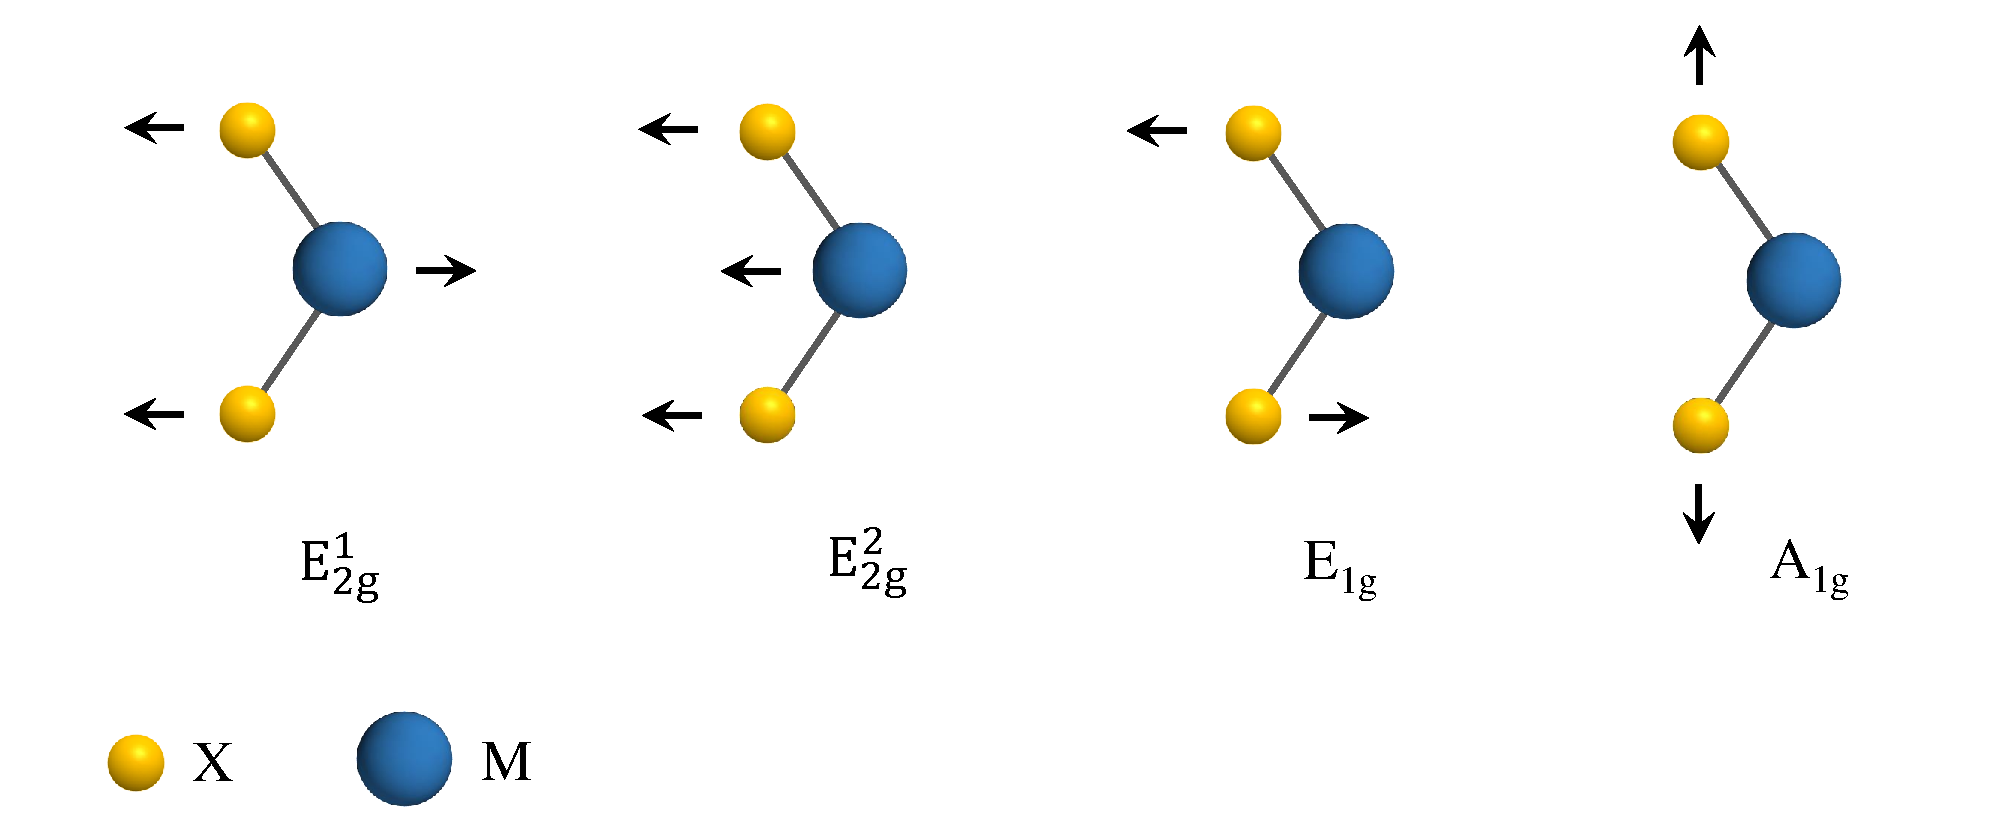
\includegraphics[width=1\textwidth,keepaspectratio=true]{Images/Ramanmoden.pdf}
	\caption[]{Second nice figure: Sketch of the atomic displacement for the Raman active phonon modes at the $\Gamma$-point in the monolayer $D_{3h}^1$ symmetry.}
	\label{fig:ramanmodes}
\end{figure}

\unpacklipsum[2-3]{}\lipsumexp

\newpage

\section{The second section}\label{sec:the_sec_sec}

\unpacklipsum[3]{}\lipsumexp

\subsection{Equations and referencing}\label{subsec:formulas}

In the following we show Equations \ref{eq:fractions_propto_exp} to \ref{eq:sig_ext}. You should look at \autoref{eq:polarisation}!

\begin{equation}\label{eq:fractions_propto_exp}
	\frac{I\left(A^-\right)}{I\left( A\right)}
	=\frac{\Gamma_{\text{A}^-}N_{\text{A}^-}}{\Gamma_\text{A}N_{\text{A}}}\propto\frac{\Gamma_{\text{A}^-}}{\Gamma_{\text{A}}}\frac{1}{n_e}\exp{\left(\frac{\text{E}_{\text{A}^-}}{k_{\text{B}}\text{T}}\right)}
\end{equation}

\begin{equation}\label{eq:oplus}
	\Gamma=A_{1g}\oplus 2A_{2u}\oplus B_{1u}\oplus 2B_{2g}\oplus E_{1g}\oplus 2E_{1u}\oplus E_{2u}\oplus 2E_{2g}.
\end{equation}

\begin{equation}\label{eq:permittivity}
	m^*\dfrac{d^2x}{dt^2}+\dfrac{m^*}{\tau}\dfrac{dx}{dt}=-eE_0e^{-i\omega t}.
\end{equation}

\begin{equation}\label{eq:solution_Drude}
	x(t)=\dfrac{e}{m^*}\dfrac{1}{\omega(\omega +i\frac{1}{\tau})}E_0e^{-i\omega t}
\end{equation}

\begin{equation}\label{eq:polarisation}
	\textbf{P}=\epsilon_0\chi \textbf{E}=n_V\textbf{p}_{\text{el}},
\end{equation}

\begin{equation}\label{eq:approx_permittivity}
\varepsilon_r(\omega)\approx 1-\dfrac{\omega_p^2}{\omega^2},~~~~\varepsilon_i(\omega)\approx \dfrac{\omega_p^2}{\omega^3}\Gamma.
\end{equation}

\begin{align}
	\sigma_{\text{ext}}&=\dfrac{2\pi}{|\textbf{k}|^2}\sum\limits_{L=1}^{\infty}(2L+1)\text{Re}\left\lbrace a_L+b_L \right\rbrace\label{eq:sig_ext_sum}\\
	\sigma_{\text{sca}}&=\dfrac{2\pi}{|\textbf{k}|^2}\sum\limits_{L=1}^{\infty}(2L+1)(|a_L|^2+|b_L|^2)\label{eq:sig_sca_sum}\\
	\sigma_{\text{abs}} &=\sigma_{\text{ext}}-\sigma_{\text{sca}}\label{eq:sig_abs}
\end{align}

We can even cite the equations in the align environment above. Like \autoref{eq:sig_ext_sum} and \autoref{eq:sig_sca_sum}

\begin{equation}\label{eq:sig_ext}
	\sigma_{\text{ext}}=12\pi\epsilon_m^{3/2}R^3\dfrac{\omega}{c}\dfrac{\varepsilon_i(\omega)}{\left[\varepsilon_r(\omega)+2\epsilon_m\right]^2+\varepsilon_i(\omega)^2},
\end{equation}

\subsection{Citation}\label{subsec:more_theory}

We will cite a lot in a theory chapter, but the best source is \autocite{gross_festkorperphysik_2018} but of course we cannot forget about \cite{fox_optical_2010,fox_quantum_2006}!

\unpacklipsum[4]{}\lipsumexp
